This chapter covers the design of the system. First, we will discuss the overall architecture of Makahiki. Then, we will describe the supporting components of the system. Finally, we will go into the top-level pages of the system.

\section{Architecture}
\label{makahiki:architecture}

\begin{figure}[h]
  \center
  \includegraphics[width=0.4\textwidth, angle=90]{images/makahiki-architecture.eps}
  \caption{Architecture of Makahiki}
  \label{fig:MakahikiArchitecture}
\end{figure}

Figure \ref{fig:MakahikiArchitecture} provides an overview of the different components of Makahiki and how they interoperate. The web application component of Makahiki is implemented using the Django web framework in the Python programming language. In addition to the modules we created, we used other third party libraries including ``django\_cas'' (an authentication plugin that allows players to authenticate using a Common Authentication Service server), ``brabeion'' (a Django module for badges), ``minidetector'' (detects if a client is a mobile phone), and ``restclient'' (a library for interacting with RESTful web services). To handle server loads more efficiently, we used memcached (an in-memory caching system) to cache parts of the website for quicker access. Figure \ref{fig:sitemap} shows how the pages are laid out in the system.

\begin{figure}[h]
  \center
  \includegraphics[width=0.4\textwidth, angle=90]{images/sitemap.eps}
  \caption{Sitemap of the pages in Makahiki}
  \label{fig:sitemap}
\end{figure}

The energy data is handled by another system called WattDepot. More details will be provided in \autoref{pages-golow:wattdepot}.

\section{Supporting Components}
\label{makahiki:components}

Before we discuss the top level pages, there are several supporting components in Makahiki. Some of these components have a UI component, while others operate behind the scenes.

\subsection{Rounds}

As part of the configuration for Makahiki, a competition period can be split up into rounds. The energy usage and points during a round are tracked separately but still contribute to the overall totals. If there is no round configured during the competition period, then the overall score is tracked. As an example, the 2011 Kukui Cup was three weeks and had two week long rounds (Round 3 was the overall round). This configuration had the interesting side effect of putting the top players in Round 1 at a disadvantage during Round 2, since they have completed most of the content that is available to them. Players who were new to the competition in Round 2 could also complete tasks that were available in Round 1, although they did miss out on any real world events and excursions that happened during that time.

\subsection{First Login Wizard}
\label{makahiki:components-setup}

\begin{figure}[h]
  \center
  \includegraphics[width=0.4\textwidth]{images/first-login-terms.eps}
  \caption{Terms and conditions step in the first login wizard.}
  \label{fig:first-login-terms}
\end{figure}

When a player logs in to the site for the first time, they are taken to the First Login Wizard. Inspired by the setup processes for other websites, the First Login Wizard guides the player through setting up their profile and getting them acclimated to the competition. \autoref{fig:first-login-terms} shows the terms and conditions step of the first login wizard. The First Login Wizard is split up in to 7 steps.

\begin{enumerate}
    \item Welcome: This also shows the player their configured name and floor. If this is not correct, they are asked to email the competition organizers.
    \item Terms and Conditions: This is where organizers will place their terms and conditions. Players are given the option to not agree, in which case they will be logged out of the system.
    \item Referral Bonus: Detailed in \autoref{makahiki:components-bonuses}.
    \item Profile Setup: Here, the player can customize their user avatar and their profile name. Players can either upload a picture or use their picture from Facebook. After completing this step, the player is automatically awarded five points.
    \item Intro Video: Competition organizers can provide a video for players to view when they come to the website for the first time. This video is often linked to a task in the Smart Grid Game.
    \item Question: Organizers can provide a multiple choice question for new players to answer related to the video they just viewed. Players that answer the question correctly are awarded points corresponding to the value of the related task and the task is marked as completed. Players that do not answer correctly can complete the task later on.
    \item Success: Tells the player that the wizard is complete. This step also provides some information about the quest system, which will be discussed in \autoref{makahiki:components-quests}.
\end{enumerate}

\subsection{Quests}
\label{makahiki:components-quests}

\begin{figure}[h]
  \center
  
\includegraphics[width=0.8\textwidth]{images/quest-bar-final.eps}
  \caption{The final version of the quest bar.}
  \label{fig:quest-bar-final}
\end{figure}

One of the main challenges in Makahiki is providing guidance to new players.  When new players come to the Makahiki website, they are thrust into an unfamiliar system and have to figure out where to start or what to do next.  Most games these days contain some sort of ``tutorial'' system that help players get accustomed to the controls and the different things they have access to.  While the control system of Makahiki is straightforward (point and click), we do want to guide players to the different sections of the site so that they can become experienced players of the system.

Quests are our solution to the tutorial/help problem.  Quests are ``meta-level'' activities in that they are tasks designed to show the player the different components of the system and how they work.  Examples of quests include ``Make a commitment'' or ``Sign up for an event''.  Users are not awarded points for these tasks, but the quests they complete are tracked and shown on their profile page.  Quests also have ``levels'', so players have to complete low level quests before moving to higher level ones.  Quests use a subset of Python in order to determine when quests are available and completed.  We implemented a set of predicates that can be used in the unlock and completion conditions.  These conditions are checked as the user navigates around the site. A list of the possible quest predicates are listed in \autoref{table:quest-predicates}.

\begin{table}[t!]
	\begin{tabular}{| l || p{11cm} |}
		\hline
		Predicate & Description \\
		\hline
		has\_action & Takes an action's name as a parameter or an action's type. If the name of the action is provided, then this predicate is true if the user has submitted anything for that action. If the type is provided, then the predicate is true if the user has submitted an action with that type. Actions are described in \autoref{makahiki:pages-getnutz}. \\
		completed\_action & Also takes an action's name or an action's type as a parameter. If the name of the action is provided, then this predicate is true if the user has completed the action. If the type is provided, then the predicate is true if the user has completed an action with the given type.\\
		num\_actions\_completed & Takes a number of actions and optional category name and type parameters. The predicate is true if the user has completed at least the number of actions. If the category name parameter is provided, then the predicate will look for actions in the provided category. If the type parameter is provided, then the predicate will look for actions of the given type.\\ 
		has\_points & Takes a point value and an optional round name parameter. This predicate is true if the user has at least the number of points in their score. If the optional round name is provided, then this predicate only considers their score within that round.\\
		allocated\_ticket & Takes no parameters and is true if the user has allocated any tickets in the Raffle Game (discussed in \autoref{pages-prizes:raffle}).\\
		badge\_awarded & Takes a badge name as a parameter. The predicate is true if the user has the badge.\\
		posted\_to\_wall & Takes no parameters and is true if the user has ever posted on their floor's wall.\\
		set\_profile\_pic & Takes no parameters and is true if the user has uploaded a profile picture or used their picture from Facebook.\\
		\hline
	\end{tabular}
	\caption{Quest predicates used in Makahiki}
	\label{table:quest-predicates}
\end{table}

\subsection{Social and Referral Bonuses}
\label{makahiki:components-bonuses}

\begin{figure}[h]
  \center
  \includegraphics[width=0.4\textwidth]{images/social-bonus.eps}
  \caption{Social bonus for making a commitment.}
  \label{fig:social-bonus}
\end{figure}

In an effort to get more people to participate in the competition, we implemented two types of bonuses; social and referral. These bonuses were designed to tie into the law of intensity and is intended to get people playing with their friends. The social bonus is an administrator option when a task is created in the Smart Grid Game. It awards extra points if the player has done the task with someone else. Examples of actions with social bonus include attending an event, recording a song related to energy, or measuring a shower water flow rate. When a player submits a response for a task with a social bonus, the player can provide the email address of the person who jointly completed the task. Once the other player completes the task, the social bonus is awarded. Social bonuses are not bi-directional; if the second player doesn't provide the first player's email address, only the first player will get the social bonus. \autoref{fig:social-bonus} is what a user would see when completing a commitment with a social bonus.

\begin{figure}[h]
  \center
  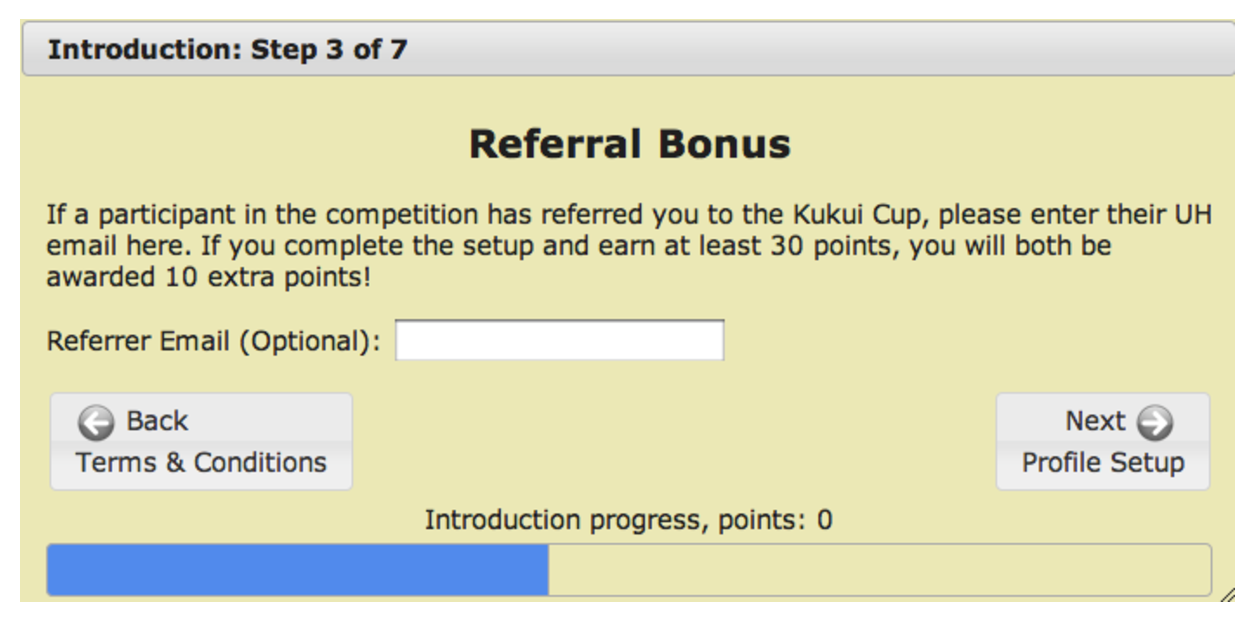
\includegraphics[width=0.4\textwidth]{images/referral-bonus.eps}
  \caption{Referral bonus step of the first login wizard.}
  \label{fig:referral-bonus}
\end{figure}

Players are led through a setup process when logging into Makahiki for the first time. One of the steps in this process is the referral bonus. If a player was referred by another player in the system, they can use this step to input their email address. Once the new player earns 30 points in the competition, both players are awarded a referral bonus of 10 points. Typically, going through the setup process gives the player fewer than 30 points, so we wanted to encourage the new player to complete at least one additional task in order to get the referral bonus. \autoref{fig:referral-bonus} shows the referral bonus step of the first login wizard.

\subsection{Badges}
\label{makahiki:components-badges}

\begin{figure}[h]
  \center
  \includegraphics[width=0.4\textwidth]{images/badges.eps}
  \caption{List of available badges in Makahiki.}
  \label{fig:badges}
\end{figure}

Web sites that incorporate concepts from gamification typically involve ``badges'', which are given to the user when they perform certain tasks within the web site. For example, the location-based social networking site ``Foursquare'' gives players badges as they visit places in their area. An example of a badge in Foursquare is the ``Gym Rat'' badge, which is given to players who visit a gym 10 times in a month. Badges can be used to provide players with additional incentive to try out new things. 

We implemented badges in Makahiki with the help of ``brabeion'', an open-source badges plugin for Django. On the player's profile page, they can view their current badges and also view the list of available badges. Additionally, in the floor's player directory, every player has their badges shown next to their name. We implemented three badges:

\begin{itemize}
    \item Daily Visitor: Awarded to a player when they visit the site three days in a row.
    \item Fully Committed: Awarded to a player when the commit to the maximum number of commitments.
    \item Bug Hunter: Awarded to a player when they report a bug in the software.
\end{itemize}

\autoref{fig:badges} is what a user sees when looking at the list of badges. The Daily Visitor badge and the Fully Committed badges are awarded automatically by Makahiki. The system checks the conditions for unlocking the badge as they perform the actions required to have them awarded. The Bug Hunter badge is awarded by a competition administrator. If an admin feels that a player deserves this badge, they can run a command on the server to give the player the badge.

\subsection{Logging}
\label{makahiki:components-logging}

Because Makahiki is developed primarily for research, we need to log user interactions with the system in order to evaluate the game design and gain insight into the players. In a production environment, the web server will log the actions of individuals when they visit the site. However, the amount of information provided by the web server is insufficient for our needs. First, the web server can only identify the player through the use of an IP address. Since first year students are likely to use more than one computer or device to access Makahiki, we need to detect those users as well. Also, when a player submits a form via a POST request, the web server does not display the contents of the submission. The information the player submitted may be lost unless we can capture their submission. Finally, many interactions in Makahiki happen through the use of Javascript. Because these actions may not trigger a request to the server (unless they use AJAX to get and retrieve data), these interactions also would not be logged.

We implemented a logging component in Makahiki to capture more complete data about the player's interaction with the website. Similar to the log format used by web applications, Makahiki's logging component captures the date and time of the request, the player's username, the type of request they made (POST, GET, etc.), the url they requested, and any POST parameters they may have submitted. To support the logging of Javascript actions in the website, the client-side Javascript can send a request to the server through a log url. This log url contains the type and id of the object they are manipulating (for example, the quest they are viewing) as well as an action. Below is an example entry in the logs.

\begin{quote}INFO 2011-10-17 00:28:17 12.223.124.27 gelee GET /home/setup/profile/ 200 \end{quote}

In addition to the request-level logging framework, the system also tracks transactions involving points in the competition. There is the potential for bugs to affect the scores of individuals in the competition. Using the log of points transactions, we can verify that the point values for individuals are correct. These actions are also helpful for players who may want more information about the things they completed. These points transactions are also displayed on the player's profile page for them to see.

Note that Makahiki's logging is provided in addition to the logging already done by the web server. Web servers can provide additional information that may be of interest to researchers looking at the data, like what browser the player used and what HTTP response code was sent back by the server.  Using these logs, researchers have a complete record of the competition.

\section{Pages}

\subsection{Get Nutz}
\label{makahiki:pages-getnutz}

\begin{figure}[h]
  \center
  \includegraphics[width=0.4\textwidth]{images/getnutz.eps}
  \caption{The Get Nutz page.}
  \label{fig:get-nutz-page}
\end{figure}

The ``Get Nutz'' page is where users come to complete \emph{actions} in order to earn points.  The main component of the page is the ``Smart Grid Game'' (SGG).  Each individual action is either locked or unlocked.  This means that some actions in the SGG are not immediately accessible by the user; they have to complete other actions in order to access them.  The SGG organizes these actions into \emph{categories}. Each category represents a column in the grid. To support this, we implemented a set of predicates that can be used to determine if a task is available or not. Examples of predicates include completing certain actions, completing actions within a category, and time-based unlocking (task is available after a certain date).

These predicates are implemented using a limited subset of Python and can be changed within the Django admin interface. Competition designers can use logical operators to combine predicates in order to organize the player's path through the Smart Grid Game. A list of predicates is shown in \autoref{table:activity-predicates}.

\begin{table}[t!]
	\begin{tabular}{| l || p{11cm} |}
		\hline
		Predicate & Description \\
		\hline
		completed\_all\_of & Takes a category name as a parameter and is true if the user has completed all of the actions in the category.\\
		completed\_some\_of & Takes a number and a category name as parameters. This predicate is true if the user has completed the number of actions in the category.\\
		completed & Takes a task name and is true if the user has completed the task.\\
		after\_published & Takes no parameters and is true if the action's publish date has passed.\\
		\hline
	\end{tabular}
	\caption{Activity predicates used in Makahiki}
	\label{table:activity-predicates}
\end{table}

There are three different types of actions in the Smart Grid Game: activities, events/excursions, and commitments. The following subsections will go into those in more detail.

\subsubsection{Activities}
\label{pages-getnutz:activities}

\begin{figure}[h]
  \center
  \includegraphics[width=0.4\textwidth]{images/activity.eps}
  \caption{A activity in the Smart Grid Game.}
  \label{fig:activity-sgg}
\end{figure}

Activities are actions that require a competition participant to perform a specific action in order to earn points.  Examples of activities include attending presentations, watching energy conservation related videos, or joining campus sustainability groups.  These activities are designed to make participants more knowledgeable and get them involved with the sustainability community. \autoref{fig:activity-sgg} shows a video in the SGG that helps people learn how to play the game.

Users who participate in activities usually require administrator approval before they can earn the points in the activity.  Administrators can either approve or reject these requests for points.  Makahiki supports four different confirmation types: question and answer, confirmation code, image upload, and free response.

In the question and answer, the activity creator needs to come up with at least one question to ask participants.  The admin also specifies an answer to each question, which is merely used to tell administrators what the expected answer is.  When a participant requests to receive points for a question and answer activity, a random question is picked from the list of questions for that activity.  Once a participant submits their answer, it is then available for admins to review.  Activities that require participants to watch a video might require them to answer a question.  Questions can be as simple as ``What is the unit of measurement for household energy?''

A confirmation code is typically used for activities that require attendance of an event.  This will be covered more in depth in \autoref{pages-getnutz:events}.

The image upload confirmation type requires participants to upload a picture in order to verify that they have performed the activity.  When the admin creates the activity, they also specify what the content of the image should be.  After the participant performs the activity, they are asked to upload the image.  Admins can then review the image.  An activity that might require an image upload would be ``Replace an incandescent bulb with a CFL''.  The participant could then be required to take a picture of themselves holding both the CFL and the incandescent bulb.

The free response confirmation type presents a simple prompt similar to that of the question and answer.  Unlike a question and answer, however, there may be no ``correct'' answer to the prompt.  For example, a free response activity  may ask the user to perform an energy audit and provide their results.

\subsubsection{Events/Excursions}
\label{pages-getnutz:events}

\begin{figure}[h]
  \center
  \includegraphics[width=0.4\textwidth]{images/event-excursion.eps}
  \caption{A excursion in the Smart Grid Game.}
  \label{fig:excursion-sgg}
\end{figure}

Events require players to attend a presentation or workshop in order to earn points.  Excursions are similar to events, but they may require more time and are held off-campus.  Each event and excursion specify a event location and time as well as how long the excursion is expected to take.  Before an event or excursion, players have the option to sign up for it beforehand.  Players who do this will receive a 2 points as a ``signup bonus''.  These points are removed if the player later decides they are not interested in the event or excursion.  Not only does this encourage players to sign up for things they are interested in, but it can also be used by administrators to gauge interest in events and make the appropriate preparations.  We also implemented a reminder system for excursions and events, so users can receive emails and/or text messages before the event takes place. \autoref{fig:excursion-sgg} shows the PedalPalooza excursion after the excursion has occurred.

Events and Excursions are typically used with the confirmation code confirmation type.  When creating the event or excursion, the admin needs to specify the number of confirmation codes to generate.  Once the admin creates the event/excursion, they can view the list of codes generated for this activity in a printable format.  When the event occurs, competition organizers can then hand out the confirmation codes to attendees of the event who are also participating in the competition.  When a participant requests points for this activity, they are required to enter a confirmation code.  If the code is valid, it is immediately approved.  Codes cannot be used more than once and a user can only use one code per activity.

Since Events and Excursions occur at a specified date and time, players may want to be reminded when it will occur. Players can set up a reminder before the Event/Excursion occurs by providing a email address and/or a cell phone number and carrier (for text messages). These reminders can be sent up to 5 hours before the Event/Excursion takes place. A periodic script is run to send any reminders that need to be sent out at a given time.

\subsubsection{Commitments}
\label{pages-getnutz:commitments}

\begin{figure}[h]
  \center
  \includegraphics[width=0.4\textwidth,angle=270]{images/commitment.eps}
  \caption{A commitment in the Smart Grid Game.}
  \label{fig:commitment-sgg}
\end{figure}

Unlike activities, where a task is completed for points, commitments are more of a ``pledge'' to perform a task over a longer period of time.  Examples of commitments include ``Turn off the lights in the bathroom when no one is using it'' or ``Make sure the lounge television is off when no one is there''.  Commitments provide an incentive for users to change their energy usage habits. \autoref{fig:commitment-sgg} is an example of a commitment in the SGG.

Also, unlike activities, commitments do not require administrator approval.  Because of this, there are additional constraints on commitments.  First, commitments are typically worth fewer points than activities.  Second, a user can only participate in up to five commitments, which prevents users from committing to every possible commitment.  Third, users who participate in commitments are public and displayed to fellow dorm floor residents, competition billboards, and on the web site.  Finally, participation in a commitment lasts for five days.  After this point, users can either participate in the same commitments or change to different commitments.  Commitments also have signup bonuses similar to events and excursions.  Players will receive 2 points for signing up for a commitment and will have those points removed if they cancel their commitment later on.

\subsection{Go Low}
\label{makahiki:pages-golow}

The ``Go Low'' page is where users view their power and energy information.  Here, they can also see their progress towards a daily energy goal.  These visualizations are supported by WattDepot, a system developed here at the University of Hawaii at Manoa.

\subsubsection{WattDepot Integration}
\label{pages-golow:wattdepot}

WattDepot is an open source web service that collects and stores energy usage data from meters.  The system is currently under development in the Collaborative Software Development Laboratory at the University of Hawaii at Manoa.  While instances of the service are hosted in the laboratory, organizations can choose to host their own instances.

There are several reasons why we want to support integration with WattDepot.  First, the data in WattDepot is accessible via a REST API~\cite{wattdepot-rest}, meaning that external services can easily request and retrieve data from the system.  Also, WattDepot supports near-real time (sub-minute) update intervals, which is one of the reasons why competitions that use Lucid Design Group's Building Dashboard are so successful.  With these updates, we can immediately present users with their current energy usage.  Users can then run ``experiments", like seeing what happens when someone turns off their lights.  Other freely available solutions like Google PowerMeter~\cite{google-powermeter} do not have this level of feedback.

Because WattDepot stores all of this data, Makahiki can retrieve current and historical data in order to provide visualizations.  Thus, competition participants can see how their usage has changed over time.  Administrators can also use this data to see if residents are completing energy reduction goals like reducing a floor's usage by 10 percent over a week.

However, calculations that use historical data can be computationally expensive.  For example, in order to calculate a floor's energy usage during a round, WattDepot must sum up power information for the floor over a period of time.  Given that we may have hundreds of users accessing the site at any given time, having to calculate this information repeatedly will put a burden on WattDepot.  In order to mitigate this issue, we created a cache for WattDepot data in Google Spreadsheets~\cite{wattdepot-cloud-cache}.  The spreadsheets are periodically updated by updaters running alongside WattDepot.  Then, instead of going to WattDepot directly, Makahiki will use a Google Spreadsheet URL to access the cached data.

\subsubsection{Current Power and Energy}
\label{pages-golow:current}

The left side of the ``Go Low'' page contains a power meter and the energy scoreboard.  The power meter shows the user their current power usage in their floor and is updated every 15 seconds.  The energy scoreboard shows the floor's energy usage during each round and is updated hourly.  While the energy scoreboard is not updated as frequently as the power meter, it is able to calculate historical data by using a spreadsheet that contains the energy data over the last thirty days.

\subsubsection{Daily Energy Goal Game}
\label{pages-golow:energygoal}

Competition administrators can create daily energy goals that take place over the course of the competition by creating another Google Spreadsheet.  This spreadsheet should contain a ``goal'' energy usage for the floor to attain.  The spreadsheet is then updated periodically with the floor's current energy information.  This spreadsheet is used to provide a daily energy goal widget in the ``Go Low'' page.  The stoplight in the middle of the the widget is green if the user's floor is on track toward meeting their goal, red if they are not on track, and yellow if they are close to being off track.  Note that red and yellow do not necessarily mean that the user's floor cannot meet their daily energy goal.  Informing users whether or not they are on track gives them the opportunity to adjust their energy consumption habits as necessary to meet the goal.  If the light were to turn red when they went over the goal, the members of that floor would not be able to do anything about it.

Makahiki can be configured by a daemon process (like launchd or cron) to check if floors have met their energy goal during the day.  This is accomplished using the Python GData Library provided by Google~\cite{python-gdata}.  This process goes out to the spreadsheet and compares each floor's energy usage to their goal usage.  If a floor meets their energy goal, each member of the floor that is participating in the game will receive 20 points. The Daily Energy Goal Game provides the link between the energy literacy (points) competition and the energy competition.

\begin{figure}[t!]
  \center
  \includegraphics[width=0.4\textwidth]{images/daily-energy-goal-game.eps}
  \caption{Daily Energy Goal Game visualization}
  \label{fig:DailyEnergyGoal}
\end{figure}

Figure \ref{fig:DailyEnergyGoal} shows what a player would see when they go to the energy page. The Daily Energy Goal display shows both their current progress and their goal so far for two reasons. First, everyone will be under their actual energy goal for most of the day, so this display would not be very useful. Second, we have noticed that the students in the residence halls use more energy at night rather than during the day. Thus, it is easy to be under for most of the day and then jump over the goal at the very end. Displaying their goal so far provides a pace for players to follow.

\subsection{Prizes}
\label{makahiki:pages-prizes}

The prizes page is where players can go to see the things they can win in the competition. The prizes serve as additional motivation for the Law of Readiness and encourage players to play more. There are two sub-sections of the prizes page; the competition prizes and the raffle game.

\subsubsection{Competition Prizes}

\begin{figure}[h]
  \center
  \includegraphics[width=0.4\textwidth]{images/prizes-winners.eps}
  \caption{Competition prizes displayed on the prizes page.}
  \label{fig:prizes-winners}
\end{figure}

In an energy competition, there are typically prizes for the winners. For the two competitions (points and energy reduction), we can award prizes to the floor that wins each competition. We can also award prizes to the top individuals in a floor or overall in the points competition. Finally, prizes may be given out for the winners of a round in the competition as well as the overall competition. \autoref{fig:prizes-winners} shows the list of prizes on the prizes page.

Makahiki supports these competition prizes through the use of the Django admin interface. A competition organizer needs to provide a title, description, value, the round for the prize, who the prize should be awarded to (for example, overall floor winner or individual points winner in a floor), and the competition type (either points or energy).  This information is used in the prizes page, where players can view the current prizes as well as who is in the lead for those prizes. Players can also view past prizes, and the winners of those prizes are displayed as well.

\subsubsection{Raffle Game}
\label{pages-prizes:raffle}

\begin{figure}[h]
  \center
  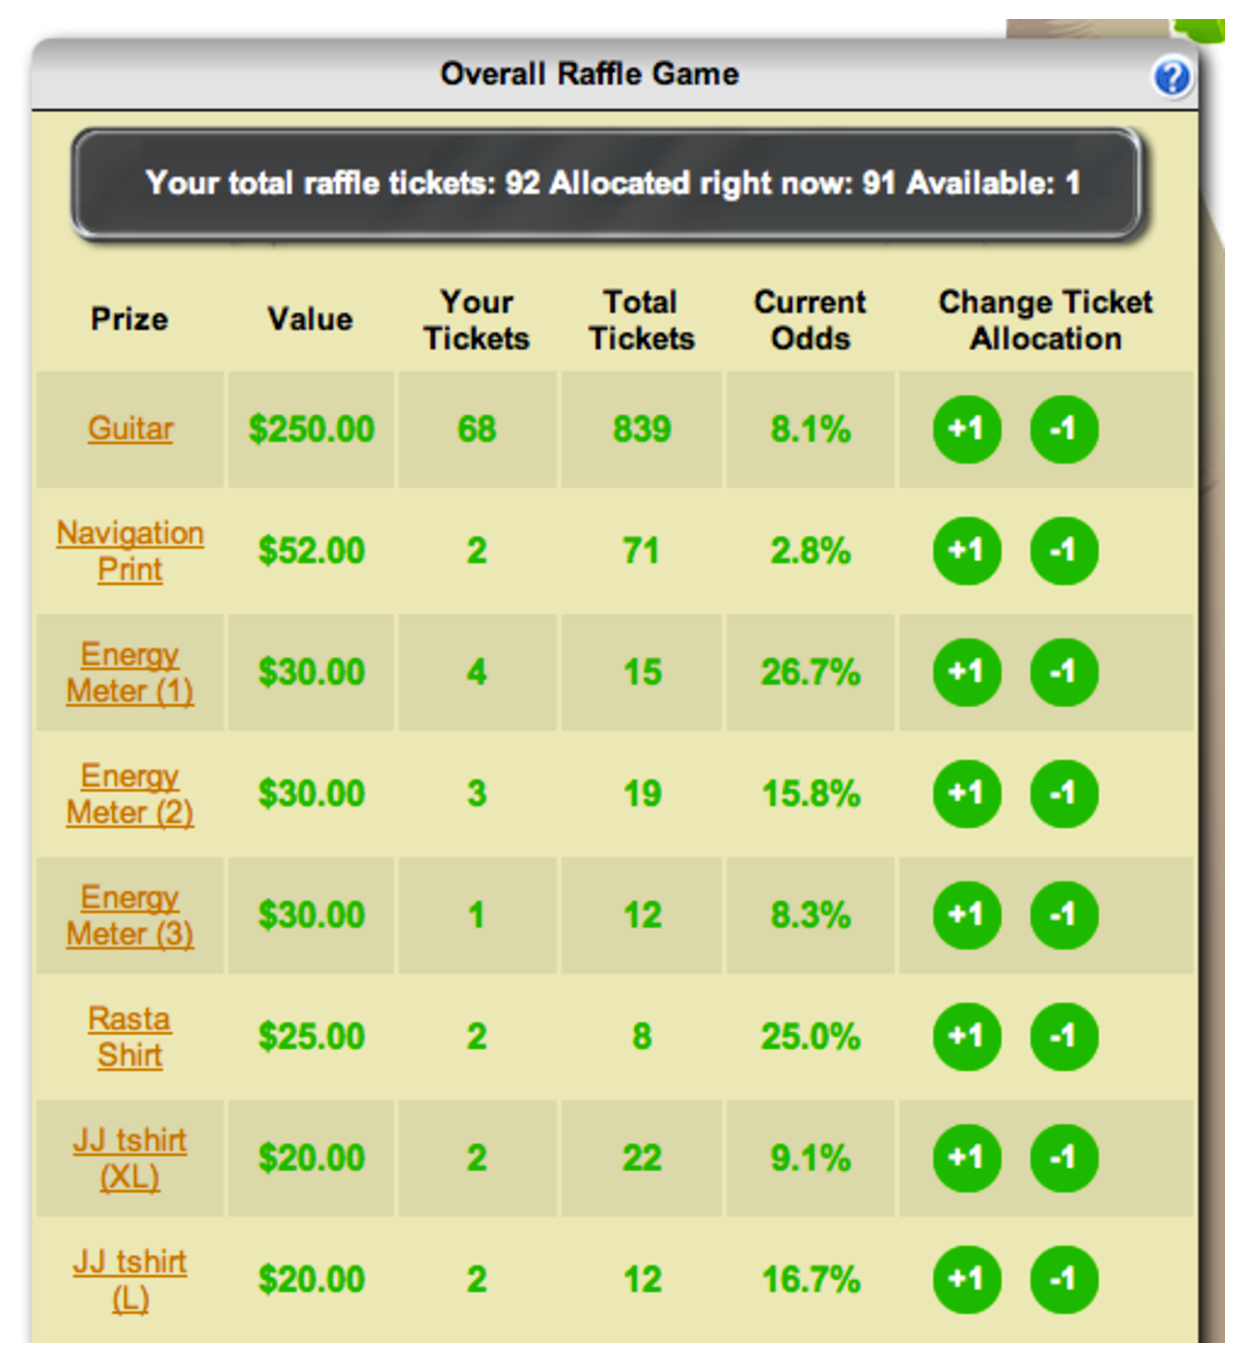
\includegraphics[width=0.4\textwidth]{images/raffle-game.eps}
  \caption{The raffle game at the end of the overall round.}
  \label{fig:raffle-game}
\end{figure}

Our initial concept of Makahiki involved awarding prizes to the top individual points getter, top lounge points getter, and the lounge that used the least energy during each round.  Players who enter the game in the middle of a round may be discouraged by the top players in that round because they will have a head start.  Since an individual prize is only awarded to the top points getter, they may feel unable to catch up and decide not to play.

To alleviate this, we came up with the Raffle.  Every 25 points a player earns in the game gets them one raffle ticket.  These raffle tickets can be used toward the prize of their choice.  Each round will have its own set of prizes and unused tickets carry over from round to round.  Winners of each prize are chosen at the end of the round.  The Makahiki website shows the player the number of tickets they allocated as well as the total number of tickets allocated for each prize.  It also shows the odds of the player winning the prize so that they can decide whether or not they want to allocate a prize or not. \autoref{fig:raffle-game} shows the raffle game at the very end of the 2011 Kukui Cup.

At first glance, this does not solve the issue of top players dominating the game.  Since these players have a lot of points, they will have a lot of raffle tickets to allocate.  However, these players will have to decide how to divvy up their tickets.  Because we show the number of tickets allocated for each prize, other players can find prizes that they have a better chance of winning.  Also, unlike the overall prizes, these raffle prizes do not have to be appealing to everyone since players can choose the prize(s) that interest them the most. On the other hand, the onus falls upon the competition organizers to get a wide selection of raffle prizes for the competition.  If there are only a few prizes for each round, then players with lots of points can dominate the raffle with their large amount of tickets.

\subsection{News}
\label{makahiki:pages-news}

\begin{figure}[h]
  \center
  \includegraphics[width=0.4\textwidth]{images/news.eps}
  \caption{The news page.}
  \label{fig:news-prod}
\end{figure}

In the context of a residence hall energy competition, players may want a place to communicate with each other. The news page provides a ``wall'' similar to the ones used by social networking websites that allow players within a floor to communicate with each other. In addition to player-provided posts, automatic posts are created as players add and/or complete actions within the competition. For example, when a player adds a commitment, an automated post is made to the floor's wall that says the player has added the commitment.

The News page also provides a ``floor directory'', where players can see what others in their floor are doing. There, the avatar, profile name, points, rank, badges, and public commitments are displayed for each member of the floor.

\subsection{Profile}
\label{makahiki:pages-profile}

\begin{figure}[h]
  \center
  \includegraphics[width=0.4\textwidth]{images/profile.eps}
  \caption{The profile page.}
  \label{fig:profile-prod}
\end{figure}

Each player has a ``profile'' that allows the player to provide an online identity within the system. Players can provide their own profile name and an avatar image. Players who want to use their picture from Facebook can link their Makahiki profile to their Facebook profile through the use of the Facebook API. Players can also set their default reminder settings (for Events and Excursions) so they do not have to enter that information every time they want to create a reminder. All of these things can be changed at any time by the player during the competition.

\subsection{Help}
\label{makahiki:pages-help}

\begin{figure}[h]
  \center
  \includegraphics[width=0.4\textwidth]{images/help.eps}
  \caption{The help page.}
  \label{fig:help-prod}
\end{figure}

The Help page is where players can go if they have questions. Competition organizers provide help topics for the Help page through the Django admin interface. In addition to the content provided by competition organizers, a form is available for players to ask the competition administrators a question. This form, when submitted, will send an email to a pre-configured email address on behalf of the player. The email will also contain the email address of the player, so a competition organizer can reply to them directly.

\subsection{Canopy}
\label{makahiki:components-canopy}

We designed the Canopy to be a place for the top players to go and view
more advanced energy visualizations and actions. Elite players could ``level
up'' and reinforce the laws of intensity and effect for learning. The current visual design of
main game has a forest background with trees, bushes, and grass. The
background of the Canopy, however, is different from the rest of the
system, with tree tops on the bottom and blue skies on top to symbolize
that the Canopy and its players are above the ``Forest'' level. Players need to be invited
to the Canopy. A competition administrator can run a command on the server
that adds the top players to the Canopy.

\begin{figure}[ht!]
  \center
  \includegraphics[width=0.6\textwidth]{images/canopy-missions-visualizations.eps}
  \caption{Canopy Missions and Visualizations}
  \label{fig:CanopyMissions}
\end{figure}

In addition to the new background, the Canopy page includes new components. First, there is a Canopy wall that members can use to communicate with other Canopy members as well as administrators (who can always access the Canopy). Second, there are Canopy missions that replace the quest interface. Unlike quests, missions do not use predicates in order to determine when they are completed. Instead, missions are completed when their related Canopy actions are completed. These Canopy actions are based on the actions in the Smart Grid game, but they do not appear in the Smart Grid. Also, some Canopy actions may require collaboration with others to complete. Finally, the Canopy includes advanced energy visualizations, which give members additional insight into how the other lounges are doing in the energy competition. Unlike the energy data displayed on other pages, these advanced energy visualizations access WattDepot's API directly. Figure \ref{fig:CanopyMissions} shows an example of a mission and an advanced energy visualization.

When we designed the Canopy, we initially thought we would provide points for completing Canopy actions. Since only elite players were invited to the Canopy, earning points would allow the top players to earn points not available to the rest of the players, allowing them to obtain an insurmountable advantage. Thus, instead of points, Canopy actions award ``Canopy Karma''. A scoreboard is shown on the Canopy page and the top Canopy player earns a prize.
